\documentclass[
11pt, % The default document font size, options: 10pt, 11pt, 12pt
english, % ngerman for German
singlespacing, % Single line spacing, alternatives: onehalfspacing or doublespacing
headsepline, % Uncomment to get a line under the header
]{MastersDoctoralThesis} % The class file specifying the document structure


\usepackage{listings}
\usepackage{xcolor}

\definecolor{dkgreen}{rgb}{0,0.6,0}
\definecolor{gray}{rgb}{0.5,0.5,0.5}
\definecolor{mauve}{rgb}{0.58,0,0.82}

\lstset{frame=tb,
  language=Java,
  aboveskip=3mm,
  belowskip=3mm,
  showstringspaces=false,
  columns=flexible,
  basicstyle={\small\ttfamily},
  numbers=none,
  numberstyle=\tiny\color{gray},
  keywordstyle=\color{blue},
  commentstyle=\color{dkgreen},
  stringstyle=\color{mauve},
  breaklines=true,
  breakatwhitespace=true,
  tabsize=3
}

\usepackage[utf8]{inputenc} % Required for inputting international characters
\usepackage[T1]{fontenc} % Output font encoding for international characters
\usepackage{float}

\usepackage{mathpazo} % Use the Palatino font by default

\usepackage[backend=bibtex,style=authoryear,natbib=true]{biblatex} % Use the bibtex backend with the authoryear citation style (which resembles APA)

\addbibresource{example.bib} % The filename of the bibliography

\usepackage[autostyle=true]{csquotes} % Required to generate language-dependent quotes in the bibliography
\usepackage{pdfpages}

%----------------------------------------------------------------------------------------
%	MARGIN SETTINGS
%----------------------------------------------------------------------------------------

\geometry{
	paper=a4paper, % Change to letterpaper for US letter
	inner=2.5cm, % Inner margin
	outer=3.8cm, % Outer margin
	bindingoffset=.5cm, % Binding offset
	top=1.5cm, % Top margint
	bottom=1.5cm, % Bottom margin
	%showframe, % Uncomment to show how the type block is set on the page
}

%----------------------------------------------------------------------------------------
%	THESIS INFORMATION
%----------------------------------------------------------------------------------------

\thesistitle{Esame di Stato 2020-2021} % Your thesis title, this is used in the title and abstract, print it elsewhere with \ttitle
\supervisor{Prof. \textsc{Luigi Menchise}} % Your supervisor's name, this is used in the title page, print it elsewhere with \supname
\examiner{} % Your examiner's name, this is not currently used anywhere in the template, print it elsewhere with \examname
\degree{Informatica} % Your degree name, this is used in the title page and abstract, print it elsewhere with \degreename
\author{\textsc{Robert-Georgian Nitu}} % Your name, this is used in the title page and abstract, print it elsewhere with \authorname
\addresses{} % Your address, this is not currently used anywhere in the template, print it elsewhere with \addressname

\subject{Informatica} % Your subject area, this is not currently used anywhere in the template, print it elsewhere with \subjectname
\keywords{} % Keywords for your thesis, this is not currently used anywhere in the template, print it elsewhere with \keywordnames
\university{\href{https://itispz.scuolainfo.it}{Einstein - De Lorenzo}} % Your university's name and URL, this is used in the title page and abstract, print it elsewhere with \univname

\AtBeginDocument{
\hypersetup{pdftitle=\ttitle} % Set the PDF's title to your title
\hypersetup{pdfauthor=\authorname} % Set the PDF's author to your name
\hypersetup{pdfkeywords=\keywordnames} % Set the PDF's keywords to your keywords
}

\begin{document}

\frontmatter % Use roman page numbering style (i, ii, iii, iv...) for the pre-content pages

\pagestyle{plain} % Default to the plain heading style until the thesis style is called for the body content

\begin{titlepage}
\begin{center}

\vspace*{.06\textheight}
{\scshape\LARGE \univname\par}\vspace{1.5cm} % University name

\HRule \\[0.4cm] % Horizontal line
{\huge \bfseries \ttitle\par}\vspace{0.4cm} % Thesis title
\HRule \\[1.5cm] % Horizontal line
 
\begin{minipage}[t]{0.4\textwidth}
\begin{flushleft} \large
\emph{Autore:}\\
\href{http://niturobert.github.io}{\authorname} % Author name - remove the \href bracket to remove the link
\end{flushleft}
\end{minipage}
\begin{minipage}[t]{0.4\textwidth}
\begin{flushright} \large
\emph{Tutor:} \\
\supname % Supervisor name - remove the \href bracket to remove the link  
\end{flushright}
\end{minipage}\\[3cm]
 
\vfill

\vfill

{\large \today}\\[4cm] % Date
%\includegraphics{Logo} % University/department logo - uncomment to place it
 
\vfill
\end{center}
\end{titlepage}


\pagestyle{thesis} % Return the page headers back to the "thesis" style

% Uncomment the lines as you write the chapters

% Chapter 1

\chapter{Task} % Main chapter title

\label{Chapter1} % For referencing the chapter elsewhere, use \ref{Chapter1} 

%----------------------------------------------------------------------------------------

% Define some commands to keep the formatting separated from the content 
\newcommand{\keyword}[1]{\textbf{#1}}
\newcommand{\tabhead}[1]{\textbf{#1}}
\newcommand{\code}[1]{\texttt{#1}}
\newcommand{\file}[1]{\texttt{\bfseries#1}}
\newcommand{\option}[1]{\texttt{\itshape#1}}

%----------------------------------------------------------------------------------------

\section*{0.1 \hspace{1cm} Translated Task}

The electricity distribution company plans to develop a digital archive of all the power lines it manages.
The digital archive must allow locating the power cabins and the pylons of the power lines.
The candidate, after formulating the appropriate additional assumptions on the characteristics and nature of the problem in question,
must identify the specifications that the system must satisfy both from the software point of view and of the network infrastructure.
Based on these specifications, illustrate some of the possible solutions, choose one, and explain why. \\

The candidate, therefore, must develop the entire project of the IT system, in particular:
the block diagram of the modules of the software product to be created;
the conceptual scheme, the logical scheme, the required DDL instructions for the implementation of the database and some required
queries for the development of the software modules identified;
the source code of a significant part of the website in a programming language chosen by the candidate.

%----------------------------------------------------------------------------------------

\section*{0.2 \hspace{1cm} Italian Version}

La società di distribuzione dell'energia elettrica intende sviluppare un archivio digitale di tutte le linee elettriche che gestisce.
Il sistema deve permettere di mappe sul territorio la collocazione delle cabine di distribuzione e dei tralicci delle linee elettriche.
Il candidato, formulate le opportune ipotesi aggiuntive sulle caratteristiche e la natura del problema in oggetto, sviluppi un'analisi della realtà di
riferimento individuando quali devono essere le specifiche che il sistema deve soddisfare sia dal punto di vista software che dell'infrastruttura di rete.
Sulla base delle specifiche individuate, illustri quali possono essere le soluzioni possibili e scegli a quella chiesto motivato giudizio è la più idonea
a rispondere alle specifiche indicate. \\

Il candidato, quindi, sviluppi l'intero progetto del sistema informatico, in particolare riportando:
lo schema a blocchi dei moduli del prodotto software da realizzare;
il progetto del database completo dello schema concettuale, dello schema logico, delle istruzioni DDL necessarie
per l'implementazione fisica del database e di alcune query necessarie per sviluppare dei moduli software individuati;
il codice di una parte significativa del software in un linguaggio di programmazione a scelta del candidato.


\definecolor{codegreen}{rgb}{0,0.6,0}
\definecolor{codegray}{rgb}{0.5,0.5,0.5}
\definecolor{codepurple}{rgb}{0.58,0,0.82}
\definecolor{backcolour}{rgb}{0.95,0.95,0.92}

\lstdefinestyle{mystyle}{
    backgroundcolor=\color{backcolour},   
    commentstyle=\color{codegreen},
    keywordstyle=\color{magenta},
    numberstyle=\tiny\color{codegray},
    stringstyle=\color{codepurple},
    basicstyle=\ttfamily\footnotesize,
    breakatwhitespace=false,         
    breaklines=true,                 
    captionpos=b,                    
    keepspaces=true,                 
    numbers=left,                    
    numbersep=5pt,                  
    showspaces=false,                
    showstringspaces=false,
    showtabs=false,                  
    tabsize=2
}

\lstset{style=mystyle}

\chapter{Analisi della Realtà} % Main chapter title
\section*{1.1 \hspace{1cm} Analisi del Problema}
Molti Paesi hanno un modo diverso per distribuire l'energia elettrica. In Italia, per esempio, la Centrale Elettrica produce energia elettrica, che è distribuita ad una Cabina Elettrica ad alta tensione attraverso le Linee Elettriche che passano per i Tralicci.
Gli Stati Uniti, però, hanno un approccio diverso:
\begin{itemize}
    \item[1.] L'elettricità è prodotta in una centrale composta da generatori i quali possono utilizzare il vento, il carbone, il gas naturale o l'acqua.
    \item[2.] La corrente viene inviata ai trasformatori i quali alzano la tensione permettendo il trasferimento su lunghe distanze.
    \item[3.] L'elettricitá passa attraverso le linee di trasmissione ad alta tensione che si estendono in tutto il paese.
    \item[4.] Il flusso di corrente raggiunge una sottostazione, dove la tensione viene abbassata in modo da poter essere distribuita su linee elettriche più piccole.
    \item[5.] Queste linee si estendono nel centro cittadino dove trasformatori più piccoli riducono nuovamente la tensione per renderla utilizzabile nelle abitazioni. Questi trasformatori più piccoli possono essere montati sui tralicci o posizionati a terra.
    \item[6.] Si collega alle case e passa attraverso un contatore che misura il consumo di ogni cliente.
    \item[7.] L'elettricità arriva al pannello di servizio il quale é fornito dell'interruttore magneto-termico che apre la rete in caso di cortocircuito, chiusura del circuito a terra o sovraccarico.
    \item[8.] L'elettricità viaggia attraverso i fili all'interno dei muri fino alle prese e passa in tutta la casa.
\end{itemize}

Date queste differenze, solo le entità comuni a tutti i Paesi verranno memorizzate:
\begin{itemize}
    \item Centrale Elettrica
    \item Traliccio
    \item Cabina Elettrica (ad alta tensione)
    \item Linea Elettrica
\end{itemize}

Il Software Permetterà agli amministratori di sistema di effettuare operazioni CRUD (Create, Read, Update e Delete) sulle entità.

\section*{1.2 \hspace{1cm} L'azienda}
L'unica cosa che sappiamo della società è che è una società di distribuzione di Energia Elettrica. Dato che la traccia la descrive come "La Società" e non ci sta una specificazione riguardanti la nazione, considero che l'azienda ha un monopolio sul mercato dell'energia elettrica nel mondo intero, semplicemente per lavorare sul worst-case ovvero la "peggior situazione" possibile. \\

Dato che non viene specificata come deve essere memorizzata la posizione delle entità, userò il sistema di coordinate GPS. \\

Siccome non viene specificato chi può accedere l'archivio, considero che solo gli amministratori di sistema possono accederci. Gli amministratori possono inserire ed eliminare i dati direttamente dalla pagina web dell'archivio, accessibile solo a loro. \\

Per fare l'autenticazione alla piattaforma, gli impiegati devono inserire le loro credenziali, e poi fare il riconoscimento facciale per confermare la loro identita'.

L'archivio sarà popolato originariamente con dati ufficiali da NASA, data.europa.eu, etc., e verranno citati nel codice sorgente. \\




\section*{1.3 \hspace{1cm} L'infrastruttura}
L'azienda ha varie sedi sparse nel mondo, i server sono collocati nel mare (\href{https://datacenterfrontier.com/microsoft-servers-in-our-underwater-data-center-are-super-reliable/#:~:text=Microsoft%3A%20Servers%20in%20Our%20Underwater%20Data%20Center%20Are%20Super%2DReliable,-By%20Rich%20Miller&text=Microsoft%20recently%20retrieved%20the%20Project,the%20Orkney%20Islands%20in%20Scotland}{come fa microsoft}) aumentando cosí l'efficenza e riducendo i costi, essi sono anche divisi in diversi sotto domini tutti connessi allo stesso database. \\
Il DBMS scelto é PostgreSQL, per la sua scalabilitá esponenziale e per il supporto alla distribuzione in piú cluster. \\

Nell'analisi del problema sono presenti diversi sottodomini,  quelli sviluppati in questo progetto sono:
\begin{itemize}
    \item https://www.electrocorp.com/
    \item https://admin.electrocorp.com/
    \item https://api.electrocorp.com/
    \item https://mail.electrocorp.com/
\end{itemize}
(www.electrocorp.com risulta giá registrato da un'azienda non affiliata con questo progetto. Per questo il dominio deve essere sovrascritto in /etc/hosts per modificare il reindirizzamento al progetto, non puó essere applicato ad una macchina esterna alla rete). \\ \\
I server utilizzano come OS SUSE Linux, una distribuzione Enterprise di GNU/Linux pensata per i server.

La rete si compone di diverse sottoreti, una per ogni cluster, tutte gestite da Kubernetes. \\
Ogni sottorete é protetta da alcune regole firewall, di seguito la lista:
\begin{center}
    \begin{tabular}{ |l|c|c|c|c|c| } 
        \hline
        \multicolumn{6}{|c|}{Firewall on www.electrocorp.com} \\
        \hline
            Number & Protocol & Source IP     & Destination IP & Destination Port & Action \\
        \hline
            4      & ALL      & 0.0.0.0/0    & 0.0.0.0/0     & 0-65535          & ACCEPT \\
        \hline
    \end{tabular}
\end{center}
    
\begin{center}
    \begin{tabular}{ |l|c|c|c|c|c| } 
        \hline
        \multicolumn{6}{|c|}{Firewall on admin.electrocorp.com} \\
        \hline
            Number & Protocol & Source IP     & Destination IP & Destination Port & Action \\
        \hline
            1      & TCP      & 172.22.3.0/24 & 172.22.4.0/24  & 5432             & ACCEPT \\
            2      & TCP      & 32.1.0.0/16   & 172.22.3.0/24  & 443              & ACCEPT \\
            3      & ALL      & 0.0.0.0/0    & 0.0.0.0/0     & 0-65535          & DROP \\
        \hline
    \end{tabular}
\end{center}

\begin{center}
    \begin{tabular}{ |l|c|c|c|c|c| } 
        \hline
        \multicolumn{6}{|c|}{Firewall on api.electrocorp.com} \\
        \hline
            Number & Protocol & Source IP     & Destination IP & Destination Port & Action \\
        \hline
            4      & ALL      & 0.0.0.0/0    & 172.22.2.5     & 0-65535          & ACCEPT \\
        \hline
    \end{tabular}
\end{center}

La sottorete 32.1.0.0/16 é gestita dalla compagnia ed é usata per permettere agli impiegati di connettersi all'area ristretta attraverso un RDP.

\begin{center}
    \begin{tabular}{ |l|c|c|c|c|c| } 
        \hline
        \multicolumn{6}{|c|}{Firewall on the DBMS cluster} \\
        \hline
            Number & Protocol & Source IP     & Destination IP & Destination Port & Action \\
        \hline
            1      & TCP      & 172.22.2.0/24 & 172.22.4.0/24  & 5432             & ACCEPT \\
            2      & TCP      & 172.22.4.0/24 & 172.22.4.0/24  & 5432             & ACCEPT \\
            3      & ALL      & 0.0.0.0/0    & 0.0.0.0/0     & 0-65535          & DROP  \\
        \hline
    \end{tabular}
\end{center}

Di seguito la configurazione dei router (firewall, port forwarding) che girano Linux.

\lstinputlisting{Code/networking.sh}

Gli host nella stessa sottorete possono solo interagire fra loro e con il DBMS cluster. \\

Questo é il docker-compose.yml, file di configurazione, che identifica anche le varie sottoreti.

\lstinputlisting{../../../project/docker-compose.yml}

... e il file /etc/hosts (C: \textbackslash Windows \textbackslash system32 \textbackslash etc \textbackslash hosts)
\lstinputlisting{/etc/hosts}

\newpage
Ed ecco lo schema di rete:
\begin{figure}[H]
    \centering
    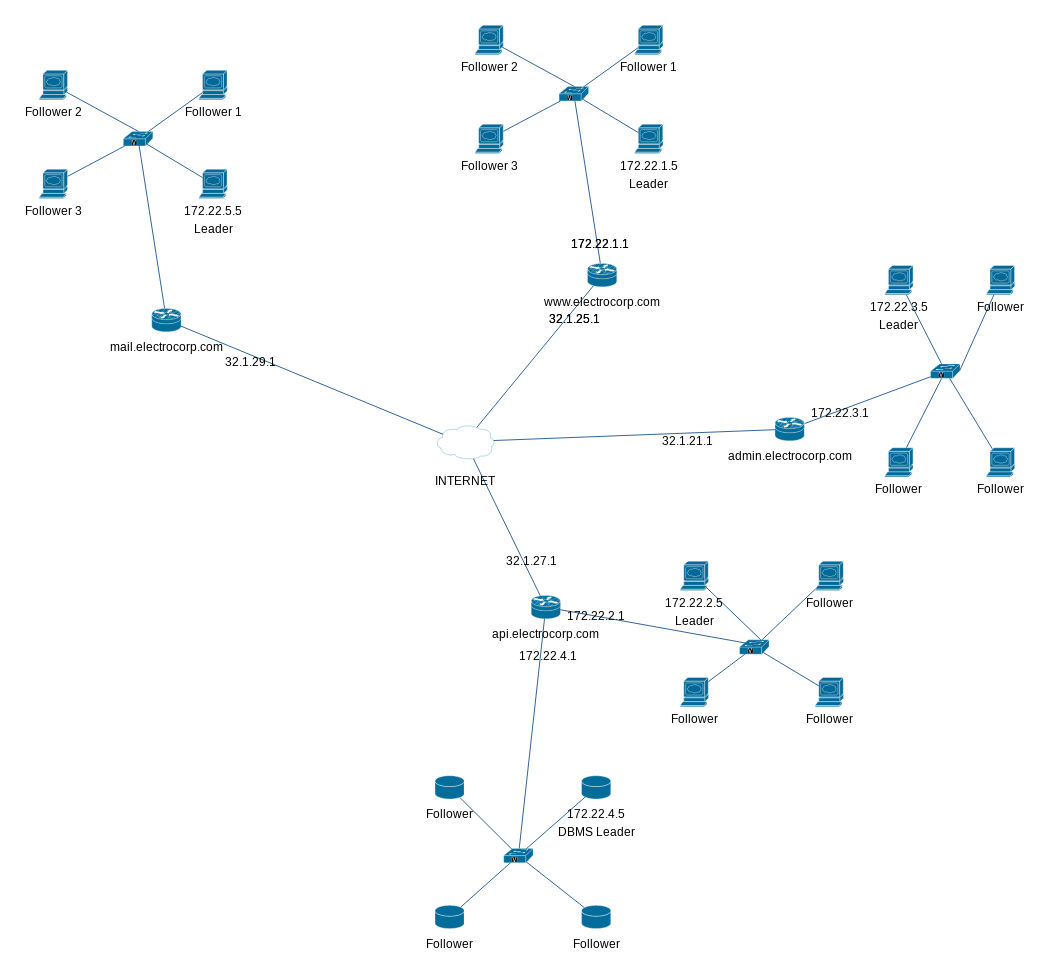
\includegraphics[width=\linewidth]{Figures/Rete.png}
\end{figure}
    
\section*{1.4 \hspace{1cm} Il sito}
Il database é accessibile solo agli amministratori di sistema, i quali possono navigare, aggiungere, eliminare e modificare i dati dallo stesso. \\

Gli amministratori di sistema possono anche gestire i ruoli e gli utenti. \\


Queste sono le regole di accesso per gli utenti su ogni sito.
\begin{center}
    \begin{tabular}{ |l|c|c|c|c|c| } 
        \hline
        \multicolumn{6}{|c|}{Access Control (admin.electrocorp.com)} \\
        \hline
                                        & Archive    & Control Panel            & Login        & Finances                & Logs \\
        \hline
            \textbf{Administrator}      & ALL        & ALL                      & AUTHENTICATE & ALL                     & READ \\
            \textbf{Finances}           &            &                          & AUTHENTICATE & ALL                     &  \\
            \textbf{*not auth*}         &            &                          & AUTHENTICATE &                         &  \\
        \hline
    \end{tabular}
\end{center}
Accessibile solo dagli impiegati. \\


Questo e' il diagramma a blocchi. \\
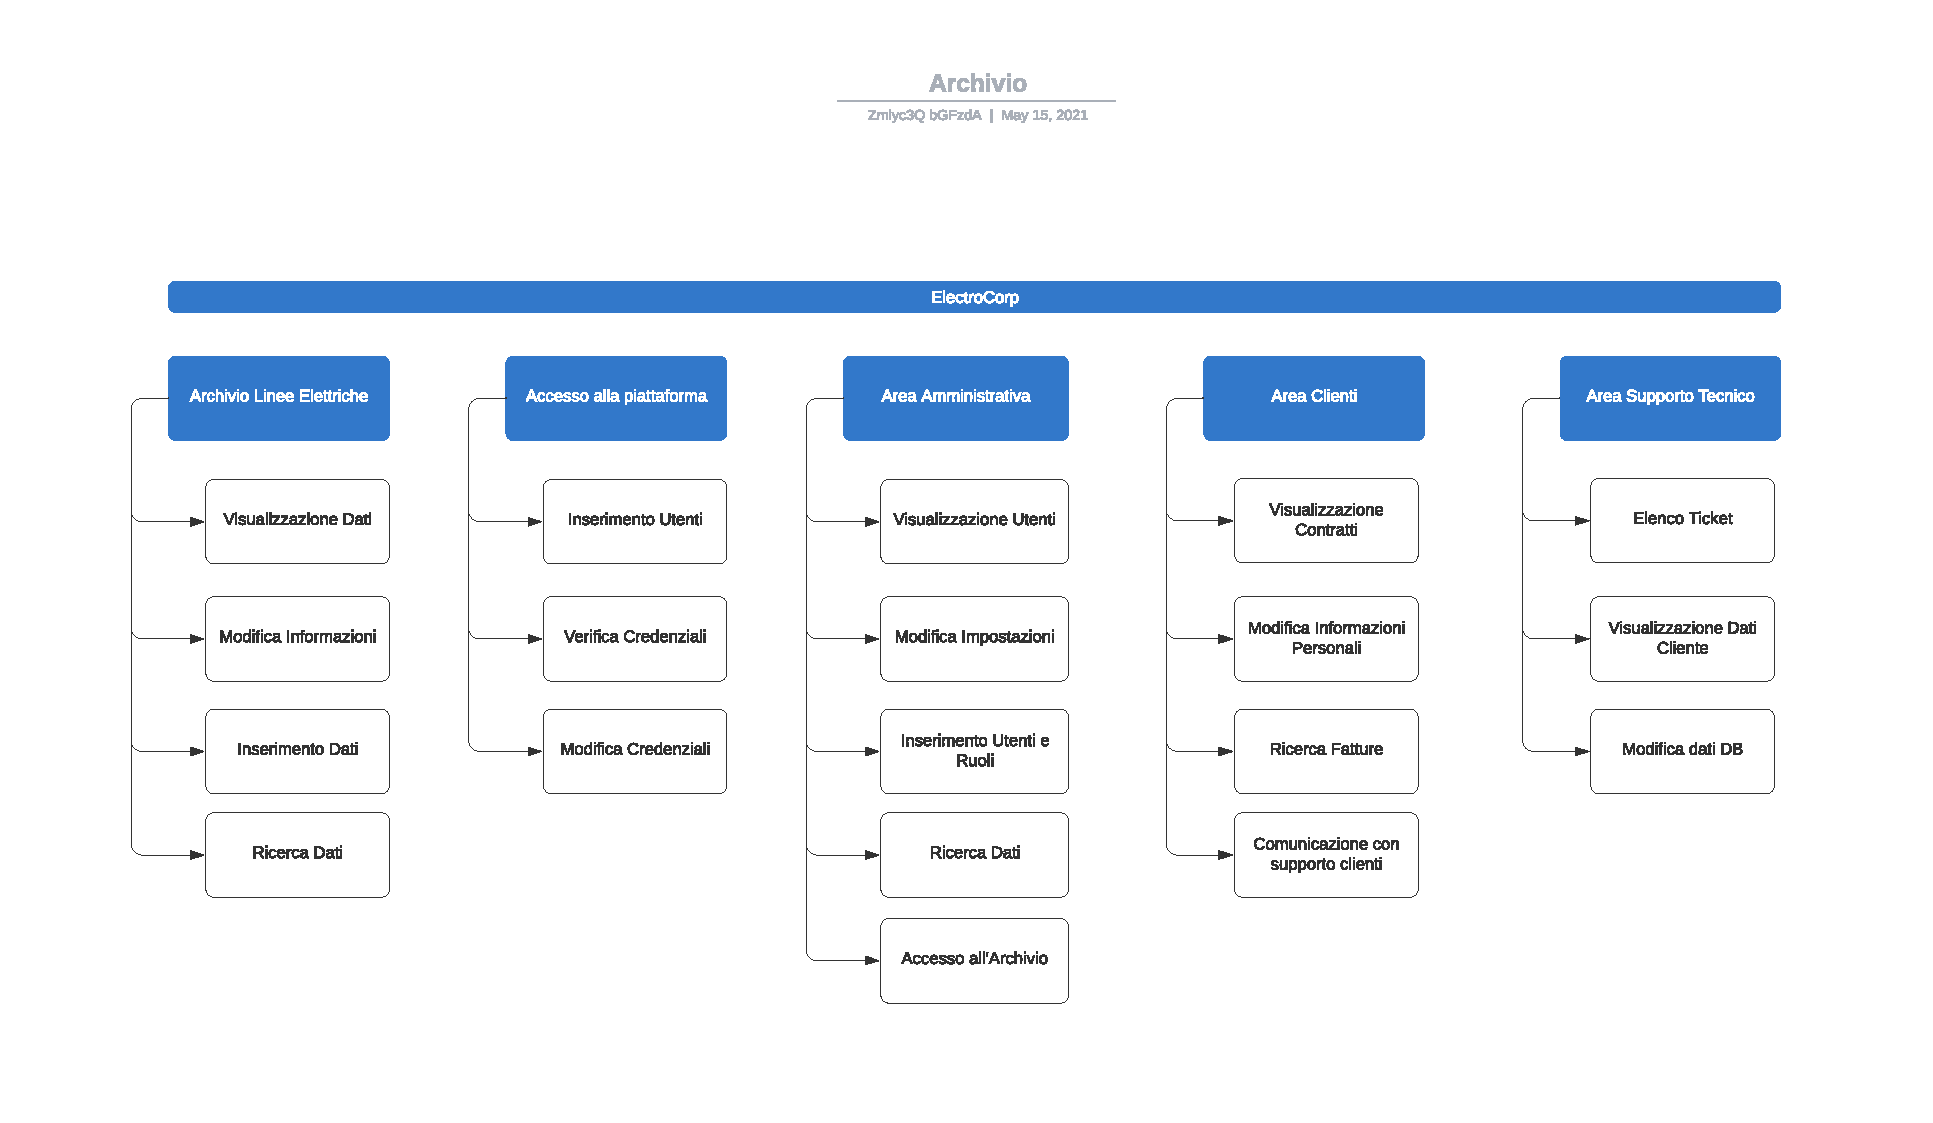
\includepdf{Figures/blocks.pdf}

E questo e' il flow chart.
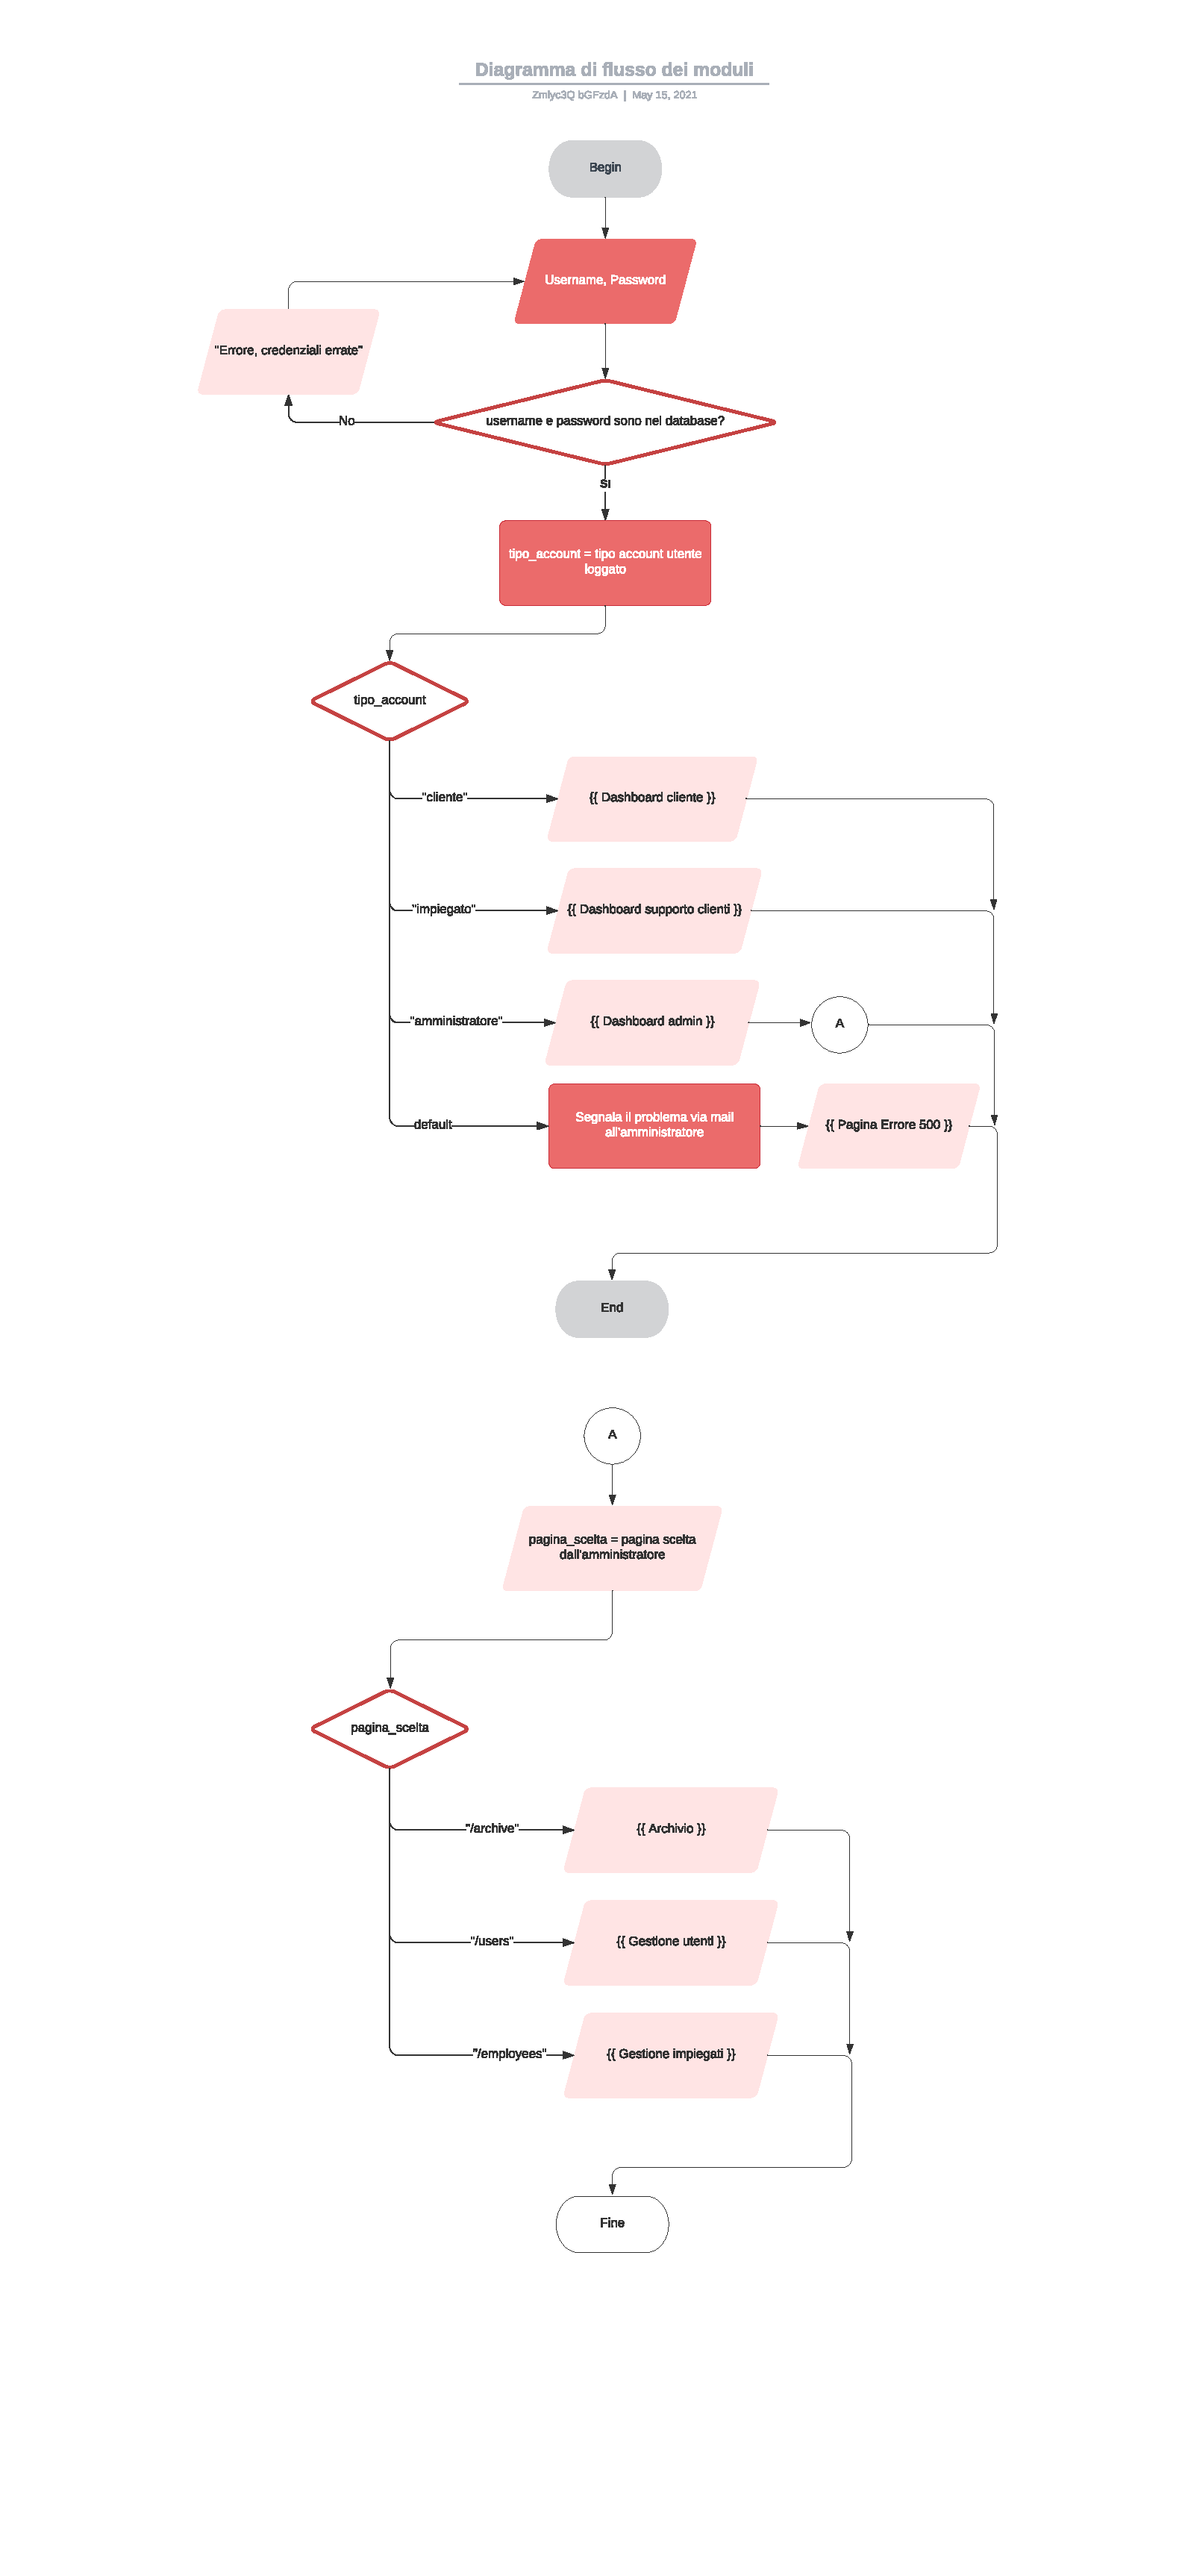
\includepdf{Figures/flow_chart.pdf}
\chapter{Full Stack Development} % Main chapter title


\section*{2.1 \hspace{1cm} Lo Stack}
\subsection*{2.1.1 \hspace{1cm} Docker}
Docker è un insieme di prodotti PaaS (Platform as a Service) che utilizzano la virtualizzazione a livello di sistema operativo per fornire software in pacchetti chiamati contenitori. I contenitori sono isolati l'uno dall'altro e raggruppano i propri software, librerie e file di configurazione; possono comunicare tra loro attraverso canali ben definiti. Poiché tutti i contenitori condividono i servizi di un singolo kernel del sistema operativo, utilizzano meno risorse rispetto alle macchine virtuali. \\

Il servizio ha livelli sia gratuito che premium. Il software che ospita i contenitori si chiama Docker Engine. È stato avviato per la prima volta nel 2013 ed è sviluppato da Docker, Inc.

\subsection*{2.1.2 \hspace{1cm} Flask su PyPy3}
Flask è un micro framework web scritto in Python. È classificato come microframework perché non richiede strumenti o librerie particolari. Non ha un livello di astrazione del database, convalida di moduli o altri componenti in cui le librerie di terze parti preesistenti forniscono funzioni comuni. Tuttavia, Flask supporta estensioni che possono aggiungere funzionalità dell'applicazione come se fossero implementate in Flask stesso. Esistono estensioni per mappatori relazionali a oggetti, convalida di moduli, gestione del caricamento, varie tecnologie di autenticazione aperta e diversi strumenti comuni relativi al framework. \\

Le applicazioni che utilizzano il framework Flask includono Pinterest e LinkedIn. \\

Flask è composto da diversi componenti, fra cui: 
\begin{itemize}
    \item \textbf{Werkzeug}: Werkzeug (termine tedesco per "strumento") è una libreria per il linguaggio di programmazione Python, in altre parole un toolkit per applicazioni WSGI (Web Server Gateway Interface), ed è concesso in licenza con licenza BSD. Werkzeug può realizzare oggetti software per funzioni di richiesta, risposta e utilità. Può essere utilizzato per creare un framework software personalizzato su di esso e supporta Python 2.7 e 3.5 e versioni successive;
    \item \textbf{Jinja}: Jinja è un motore di modelli per il linguaggio di programmazione Python ed è concesso in licenza con licenza BSD. Simile al framework web Django, gestisce i modelli in una sandbox;
    \item \textbf{MarkupSafe}: MarkupSafe è una libreria per la gestione delle stringhe per il linguaggio di programmazione Python, con licenza BSD. L'omonimo tipo MarkupSafe estende il tipo di stringa Python e contrassegna il suo contenuto come "sicuro"; la combinazione di MarkupSafe con stringhe regolari fa automaticamente l'escape delle stringhe non contrassegnate, evitando il doppio escape delle stringhe già contrassegnate;
    \item \textbf{ItsDangerous}: ItsDangerous è una libreria di serializzazione dei dati sicura per il linguaggio di programmazione Python, con licenza BSD. Viene utilizzato per memorizzare la sessione di un'applicazione Flask in un cookie senza consentire agli utenti di manomettere il contenuto della sessione.
\end{itemize}


\subsection*{2.1.3 \hspace{1cm} SQLAlchemy}
SQLAlchemy è un toolkit SQL open source e ORM (object-relational mapper) per il linguaggio di programmazione Python rilasciato sotto la licenza MIT. \\

La filosofia di SQLAlchemy è che i database relazionali si comportano meno come le raccolte di oggetti man mano che la scala diventa più grande e le prestazioni iniziano a essere un problema, mentre le raccolte di oggetti si comportano meno come tabelle e righe poiché viene progettata una maggiore astrazione. Per questo motivo ha adottato il modello di mappatura dati (simile a Hibernate per Java) piuttosto che il modello di registrazione attivo utilizzato da una serie di altri mappatori relazionali di oggetti. Tuttavia, i plugin opzionali consentono agli utenti di sviluppare utilizzando la sintassi dichiarativa. \\

SQLAlchemy è stato rilasciato per la prima volta nel febbraio 2006 ed è diventato rapidamente uno degli strumenti di mappatura relazionale a oggetti più utilizzati nella comunità Python, insieme a ORM di Django.


\subsection*{2.1.4 \hspace{1cm} PostgreSQL}
PostgreSQL, noto anche come Postgres, è un sistema di gestione del database relazionale (RDBMS) gratuito e open source che enfatizza l'estensibilità e la conformità SQL. Originariamente era chiamato POSTGRES, in riferimento alle sue origini come successore del database Ingres sviluppato presso l'Università della California, Berkeley. Nel 1996, il progetto è stato rinominato PostgreSQL per riflettere il suo supporto per SQL. Dopo una revisione nel 2007, il team di sviluppo ha deciso di mantenere il nome PostgreSQL e l'alias Postgres. \\

PostgreSQL offre transazioni con proprietà Atomicity, Consistency, Isolation, Durability (ACID), viste aggiornabili automaticamente, viste materializzate, trigger, chiavi esterne e stored procedure. È progettato per gestire una vasta gamma di carichi di lavoro, da singole macchine a data warehouse o servizi Web con molti utenti simultanei. È il database predefinito per macOS Server ed è disponibile anche per Windows, Linux, FreeBSD e OpenBSD. 

\subsection*{2.1.5 \hspace{1cm} React}
React (noto anche come React.js o ReactJS) è una libreria JavaScript front-end open source per la creazione di interfacce utente o componenti dell'interfaccia utente. È gestito da Facebook e da una comunità di singoli sviluppatori e aziende. React può essere utilizzato come base per lo sviluppo di applicazioni a pagina singola o mobili. Tuttavia, React si occupa solo della gestione dello stato e del rendering di tale stato nel DOM, quindi la creazione di applicazioni React di solito richiede l'uso di librerie aggiuntive per il routing, oltre a determinate funzionalità lato client. \\

\section*{2.2 \hspace{1cm} Il Sito}
\subsection*{2.2.1 \hspace{1cm} Il server API}
Questo è una parte del codice per il server API. \\
\lstinputlisting[language=python]{../../../project/api/code/routes.py}

Poiché abbiamo un server API (e un cluster di server), manterremo le informazioni in un token web. I token Web JSON (\ href {https://jwt.io/} {JWT}) verranno utilizzati per archiviare i dati della sessione lato client in modo sicuro. \\
Questo è il middleware per l'utilizzo di JWT. \\

\lstinputlisting[language=python]{../../../project/api/code/middleware.py}


\subsection*{2.2.2 \hspace{1cm} Il Frontend}
Entrambi i frontend di admin.electrocorp.com e (www.)electrocorp.com sono sviluppati con React.
Userò diverse librerie, fra cui:
\begin{itemize}
    \item \href{https://tailwindcss.com/}{Tailwind.css}: un framework web (tipo Bootstrap), che mi solleva dal dover scrivere un sacco di CSS e utilizzare Tailwind direttamente nella mia pagina HTML;
    \item \href{https://reactrouter.com/}{React Router}: una libreria di React.js per renderizzare più pagine nello stesso codice;
    \item \href{https://globe.gl}{Globe.gl}: una libreria di React.js per renderizzare un globo.
\end{itemize}

Questo è il codice di App.js:
\lstinputlisting{../../../project/admin/code/src/App.js}
\chapter{Amministrazione di Sistema}

\section*{3.1 \hspace{1cm} Docker Compose}
Docker Compose è uno strumento per la definizione e l'esecuzione di applicazioni Docker multi-container. Utilizza i file YAML per configurare i servizi dell'applicazione ed esegue il processo di creazione e avvio di tutti i contenitori con un unico comando. L'utilità CLIedocker-compose consente agli utenti di eseguire comandi su più contenitori contemporaneamente, ad esempio, la creazione di immagini, il ridimensionamento di contenitori, l'esecuzione di contenitori interrotti e altro ancora. I comandi relativi alla manipolazione delle immagini, o le opzioni interattive dell'utente, non sono rilevanti in Docker Compose perché indirizzano un contenitore. Il file docker-compose.yml viene utilizzato per definire i servizi di un'applicazione e include varie opzioni di configurazione. Ad esempio, l'opzione build definisce opzioni di configurazione come il percorso Dockerfile, l'opzione comando consente di sovrascrivere i comandi Docker predefiniti e altro ancora. La prima versione beta pubblica di Docker Com-pose (versione 0.0.1) è stata rilasciata il 21 dicembre 2013. La prima versione pronta per la produzione (1.0) è stata resa disponibile il 16 ottobre 2014.
\section*{3.2 \hspace{1cm} Linux}
Linux è una famiglia di sistemi operativi Unix open-source basati sul kernel Linux, un kernel del sistema operativo rilasciato per la prima volta il 17 settembre 1991 da Linus Torvalds. Linux è tipicamente impacchettato in una distribuzione Linux. \\

Le distribuzioni includono il kernel Linux e il software di sistema di supporto e le librerie, molte delle quali sono fornite dal progetto GNU. Molte distribuzioni Linux usano la parola "Linux" nel loro nome, ma la Free Software Foundation usa il nome "GNU / Linux" per enfatizzare l'importanza del software GNU, causando alcune controversie.

\section*{3.3 \hspace{1cm} iptables}
iptables è un programma di utilità per lo spazio utente che consente a un amministratore di sistema di configurare le regole del filtro dei pacchetti IP del firewall del kernel Linux, implementate come diversi moduli Netfilter. I filtri sono organizzati in diverse tabelle, che contengono catene di regole su come trattare i pacchetti di traffico di rete. Diversi moduli e programmi del kernel sono attualmente utilizzati per diversi protocolli; iptables si applica a IPv4, ip6tables a IPv6, arptables a ARP ed ebtables a frame Ethernet. \\

iptables richiede privilegi elevati per funzionare e deve essere eseguito dall'utente root, altrimenti non funziona. Sulla maggior parte dei sistemi Linux, iptables è installato come / usr / sbin / iptables e documentato nelle sue pagine man, che possono essere aperte usando man iptables una volta installato. Può anche essere trovato in / sbin / iptables, ma poiché iptables è più simile a un servizio piuttosto che a un "binario essenziale", la posizione preferita rimane / usr / sbin. 
\chapter{Moduli del Software} % Main chapter title

\section*{4.1 \hspace{1cm} Normalizzazione Database}
\subsection*{4.1.1 \hspace{1cm} Schema ER}
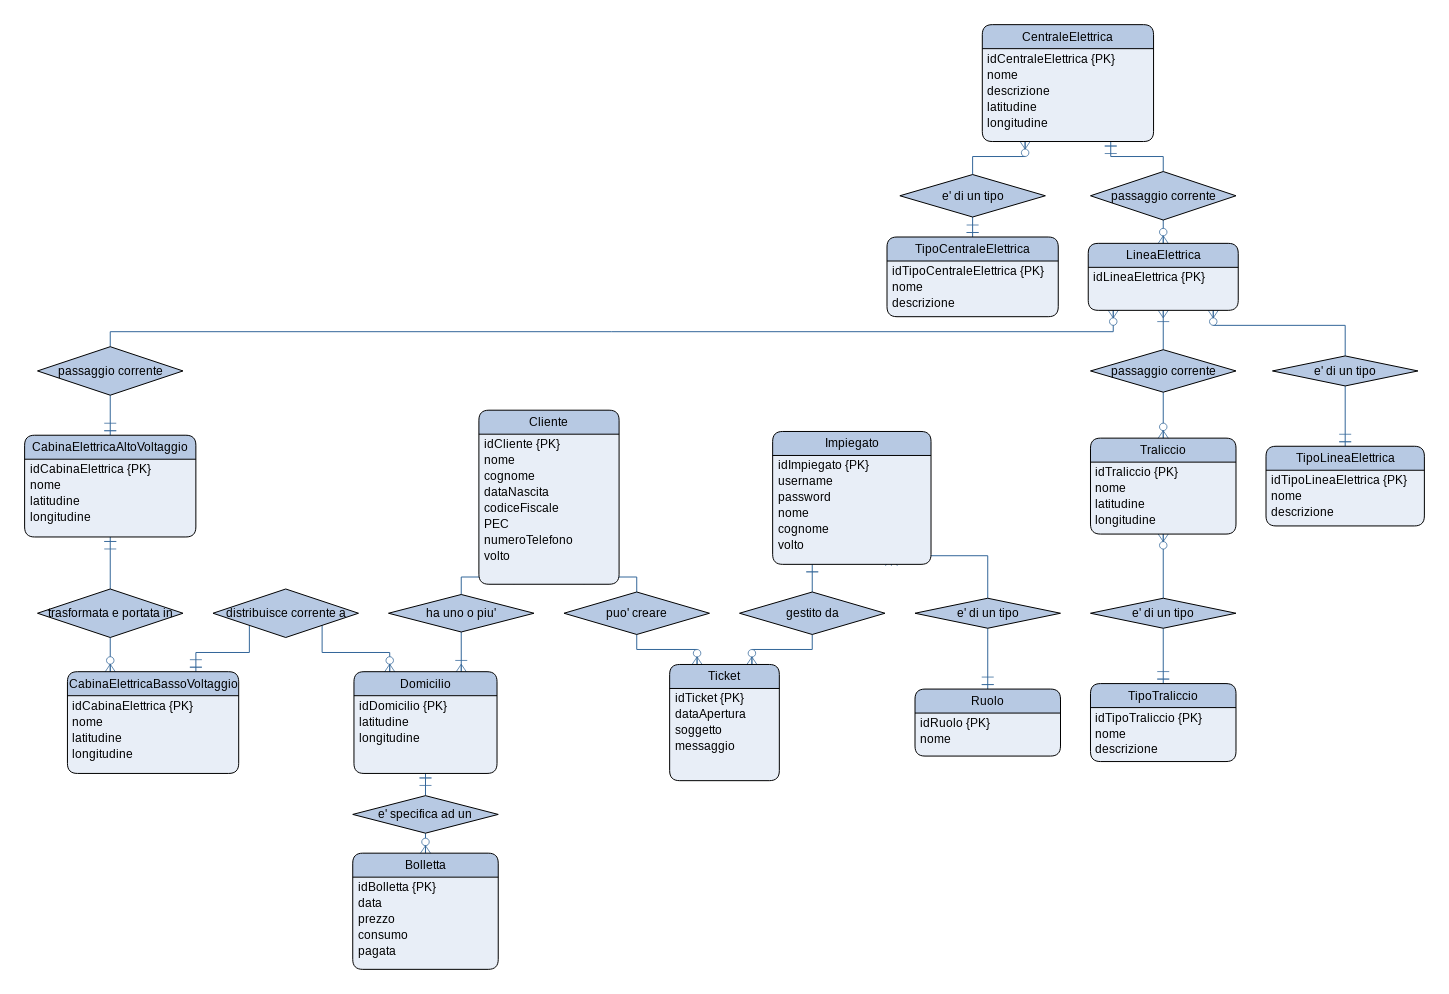
\includegraphics[width=\linewidth]{Figures/ER.png}
\subsection*{4.1.2 \hspace{1cm} 1FN}
Lo schema e' in 1a forma normale in quanto tutti gli attributi sono atomici e dello stesso tipo. \\
La prima forma normale è la più semplice, serve solo rispettare le regole di base per avere questa prima forma, le quali sono:
\begin{itemize}
    \item Utilizzo di campi elementari e non composti
    \item Stesso numero di righe e colonne
    \item Record univoci
\end{itemize}

\subsection*{4.1.3 \hspace{1cm} 2FN}
Dato che non abbiamo chiavi composte, non dobbiamo fare nulla per controllare la 2a forma normale. \\

\subsection*{4.1.3 \hspace{1cm} 3FN}
Tutte le colonne dipendono direttamente dalla chiave primaria, e' ridotto in 3a forma normale. \\

\section*{4.2 \hspace{1cm} Schema Logico}

\begin{center}
    \begin{tabular}{ |l|c|c|c|c|c|c| } 
        \hline
        \multicolumn{7}{|c|}{CentraleElettrica} \\
        \hline
            Name                    & Type      & Size  & Key       & Null  & Default   & Extra \\
        \hline
            idCentrale              & INTEGER   &       & PRIMARY   & NO    &           & AUTO INCREMENT \\
            nome                    & VARCHAR   & 128   &           & NO    &           &                \\
            descrizione             & VARCHAR   & 4096  &           & NO    &           &                \\
            latitudine              & FLOAT     &       &           & NO    &           &                \\
            longitudine             & FLOAT     &       &           & NO    &           &                \\
            idTipoCentraleElettrica & INTEGER   &       & FOREIGN   & NO    &           &                \\
        \hline
    \end{tabular}
\end{center}


\begin{center}
    \begin{tabular}{ |l|c|c|c|c|c|c| } 
        \hline
        \multicolumn{7}{|c|}{LineaElettrica} \\
        \hline
            Name                 & Type     & Size  & Key       & Null  & Default   & Extra \\
        \hline
            idLineaElettrica     & INTEGER  &       & PRIMARY   & NO    &           & AUTO INCREMENT \\
            origine              & INTEGER  &       & FOREIGN   & NO    &           & \\
            destinazione         & INTEGER  &       & FOREIGN   & NO    &           & \\
            idTipoLineaElettrica & INTEGER  &       & FOREIGN   & NO    &           & \\
        \hline
    \end{tabular}
\end{center}

\begin{center}
    \begin{tabular}{ |l|c|c|c|c|c|c| } 
        \hline
        \multicolumn{7}{|c|}{CabinaElettricaAltoVoltaggio} \\
        \hline
            Name             & Type     & Size  & Key       & Null  & Default   & Extra \\
        \hline
            idCabina         & INTEGER  &       & PRIMARY   & NO    &           & AUTO INCREMENT \\
            nome             & VARCHAR  & 128   &           & YES   &           & \\
            latitudine       & FLOAT    &       &           & NO    &           & \\
            longitudine      & FLOAT    &       &           & NO    &           & \\
        \hline
    \end{tabular}
\end{center}

\begin{center}
    \begin{tabular}{ |l|c|c|c|c|c|c| } 
        \hline
        \multicolumn{7}{|c|}{CabinaElettricaBassoVoltaggio} \\
        \hline
            Name                  & Type     & Size  & Key       & Null  & Default   & Extra \\
        \hline
            idCabina              & INTEGER  &       & PRIMARY   & NO    &           & AUTO INCREMENT \\
            nome                  & VARCHAR  & 128   &           & YES   &           & \\
            latitudine            & FLOAT    &       &           & NO    &           & \\
            longitudine           & FLOAT    &       &           & NO    &           & \\
            idCabinaAltoVoltaggio & INTEGER  &       & FOREIGN   & NO    &           & \\
        \hline
    \end{tabular}
\end{center}

\begin{center}
    \begin{tabular}{ |l|c|c|c|c|c|c| } 
        \hline
        \multicolumn{7}{|c|}{PassaggioLinea} \\
        \hline
            Name                    & Type     & Size   & Key       & Null  & Default   & Extra \\
        \hline
            idPassaggio             & INTEGER  &        & PRIMARY   & NO    &           & AUTO INCREMENT \\
            idLinea                 & INTEGER  &        & FOREIGN   & NO    & 1         & \\
            idTraliccioOrigine      & INTEGER  &        & FOREIGN   & SI    &           & \\
            idTraliccioDestinazione & INTEGER  &        & FOREIGN   & SI    &           & \\
        \hline
    \end{tabular}
\end{center}

\begin{center}
    \begin{tabular}{ |l|c|c|c|c|c|c| } 
        \hline
        \multicolumn{7}{|c|}{Traliccio} \\
        \hline
            Name             & Type     & Size  & Key       & Null  & Default   & Extra \\
        \hline
            idTraliccio      & INTEGER  &       & PRIMARY   & NO    &           & AUTO INCREMENT \\
            nome             & VARCHAR  & 64    &           & SI    &           & \\
            latitude         & FLOAT    &       &           & NO    &           & \\
            longitude        & FLOAT    &       &           & NO    &           & \\
            idTipoTraliccio  & INTEGER  &       & FOREIGN   & NO    &           & \\
        \hline
    \end{tabular}
\end{center}

\begin{center}
    \begin{tabular}{ |l|c|c|c|c|c|c| } 
        \hline
        \multicolumn{7}{|c|}{Cliente} \\
        \hline
            Name             & Type     & Size  & Key       & Null  & Default   & Extra \\
        \hline
            idCliente        & INTEGER  &       & PRIMARY   & NO    &           & AUTO INCREMENT \\
            nome             & VARCHAR  & 64    &           & NO    &           & \\
            cognome          & VARCHAR  & 64    &           & NO    &           & \\
            dataNascita      & DATE     &       &           & NO    &           & \\
            codiceFiscale    & VARCHAR  & 16    &           & NO    &           & UNIQUE \\
            numeroTelefono   & VARCHAR  & 16    &           & NO    &           & UNIQUE \\
            PEC              & VARCHAR  & 300   &           & NO    &           & UNIQUE \\
            password         & VARCHAR  & 256   &           & NO    &           & \\
            volto            & BLOB     &       &           & NO    &           & UNIQUE \\
        \hline
    \end{tabular}
\end{center}
\begin{center}
    \begin{tabular}{ |l|c|c|c|c|c|c| } 
        \hline
        \multicolumn{7}{|c|}{Domicilio} \\
        \hline
            Name             & Type     & Size  & Key       & Null  & Default   & Extra \\
        \hline
            idDomicilio                     & INTEGER  &       & PRIMARY   & NO    &           & AUTO INCREMENT \\
            idCliente                       & INTEGER  &       & FOREIGN   & NO    &           & \\
            idCabinaElettricaBassoVoltaggio & INTEGER  &       & FOREIGN   & NO    &           & \\
            latitudine                      & FLOAT    &       &           & NO    &           & \\
            longitudine                     & FLOAT    &       &           & NO    &           & \\
        \hline
    \end{tabular}
\end{center}
\begin{center}
    \begin{tabular}{ |l|c|c|c|c|c|c| } 
        \hline
        \multicolumn{7}{|c|}{Bolletta} \\
        \hline
            Name             & Type     & Size  & Key       & Null  & Default   & Extra \\
        \hline
            idBolletta       & INTEGER  &       & PRIMARY   & NO    &           & AUTO INCREMENT \\
            idDomicilio      & INTEGER  &       & FOREIGN   & NO    &           & \\
            consumoWatt      & FLOAT    &       &           & NO    & 0         & \\
            dataBolletta     & DATE     &       &           & NO    & CURDATE   & \\
            pagata           & BOOLEAN  &       &           & NO    & FALSE     & \\
        \hline
    \end{tabular}
\end{center}
\begin{center}
    \begin{tabular}{ |l|c|c|c|c|c|c| } 
        \hline
        \multicolumn{7}{|c|}{Impiegato} \\
        \hline
            Name             & Type     & Size  & Key       & Null  & Default   & Extra \\
        \hline
            idImpiegato      & INTEGER  &       & PRIMARY   & NO    &           & AUTO INCREMENT \\
            username         & VARCHAR  & 300   &           & NO    &           & UNIQUE \\
            password         & CHAR     & 128   &           & NO    &           & \\
            nome             & VARCHAR  & 64    &           & NO    &           & \\
            cognome          & VARCHAR  & 64    &           & NO    &           & \\
            ruolo            & INTEGER  &       & FOREIGN   & NO    &           & \\
            volto            & BLOB     &       &           & NO    &           & UNIQUE \\
        \hline
    \end{tabular}
\end{center}
\begin{center}
    \begin{tabular}{ |l|c|c|c|c|c|c| } 
        \hline
        \multicolumn{7}{|c|}{Ticket} \\
        \hline
            Name             & Type     & Size  & Key       & Null  & Default   & Extra \\
        \hline
            idTicket         & INTEGER  &       & PRIMARY   & NO    &           & AUTO INCREMENT \\
            dataApertura     & DATETIME &       &           & NO    &           & \\
            soggetto         & VARCHAR  & 300   &           & NO    &           & \\
            messaggio        & VARCHAR  & 8192  &           & NO    &           & \\
            idImpiegato      & INTEGER  &       & FOREIGN   & SI    &           & \\
            idCliente        & INTEGER  &       & FOREIGN   & NO    &           & \\
        \hline
    \end{tabular}
\end{center}

\section*{4.3 \hspace{1cm} DDL}
\subsection*{Metodo Tradizionale}
Questo progetto non usa il metodo "tradizionale" per creare le query SQL. \\
Di seguito, però, mostro le istruzioni DDL per creare il database. \\
\lstinputlisting[language=SQL]{Code/ddl.sql}

\subsection*{Il Metodo di SQLAlchemy}
\begin{verbatim*}
api/code/models.py
\end{verbatim*}

\lstinputlisting[language=Python]{../../../project/api/code/models.py}


Per creare le tabelle del database:
\begin{lstlisting}[language=Python]
# Da qualsiasi parte
db = SQLAlchemy(app)
db.create_db()
\end{lstlisting}


\section*{4.4 \hspace{1cm} Inserimento dei Dati}
\subsection*{Metodo Tradizionale}
\lstinputlisting[language=SQL]{Code/data.sql}

\subsection*{Il Metodo di SQLAlchemy}
\lstinputlisting[language=Python]{../../../project/api/code/data/users.py}


\section*{4.5 \hspace{1cm} Alcune query}
\subsection*{4.5.1 \hspace{1cm} Membri del team "Financing"}
\subsubsection*{Metodo Tradizionale}
\lstinputlisting[language=SQL]{Code/query-1.sql}

\subsubsection*{Il Metodo di SQLAlchemy}
\begin{lstlisting}[language=Python]
User.query.filter_by(role=Role.query.filter_by(name='Finances')[0].id)
\end{lstlisting}


\section*{4.5.2 \hspace{1cm} Centrali Elettriche rinnovabili}
\subsection*{Il Metodo Tradizionale}
\lstinputlisting[language=SQL]{Code/query-2.sql}

\subsubsection*{Il Metodo di SQLAlchemy}
\begin{lstlisting}[language=Python]
    PowerPlant.query.filter(
        PowerPlant.category.in_(
            PowerPlantCategory.query.filter_by(name='Hydro')[0].id,
            PowerPlantCategory.query.filter_by(name='Solar')[0].id,
            PowerPlantCategory.query.filter_by(name='Wind')[0].id,
            PowerPlantCategory.query.filter_by(name='Nuclear')[0].id,
            PowerPlantCategory.query.filter_by(name='Geothermal')[0].id,
        )
    )
\end{lstlisting}
 

%----------------------------------------------------------------------------------------
%	THESIS CONTENT - APPENDICES
%----------------------------------------------------------------------------------------

\appendix % Cue to tell LaTeX that the following "chapters" are Appendices

% Include the appendices of the thesis as separate files from the Appendices folder
% Uncomment the lines as you write the Appendices

% % Appendix A

\chapter{Stack} % Main appendix title

\section*{Websites}
\begin{itemize}
    \item \textbf{PyPy}: \href{https://www.pypy.org/}{Home Page}
    \item \textbf{Flask}: \href{https://flask.palletsprojects.com/en/2.0.x/}{Official Documentation}
    \item \textbf{Flask-SQLAlchemy}: \href{https://flask-sqlalchemy.palletsprojects.com/en/2.x/}{Official Documentation}
    \item \textbf{Docker}: \href{https://www.docker.com/}{Home Page}, \href{https://docker-curriculum.com/}{Unofficial Tutorial}
    \item \textbf{PostgreSQL}: \href{https://www.postgresql.org/}{Home Page}
    \item \textbf{K8S / Kubernetes}: \href{https://kubernetes.io/}{Home Page}, \href{https://kubernetes.io/docs/tutorials/kubernetes-basics/}{Official Tutorial}
    \item \textbf{React.js}: \href{https://reactjs.org/}{Home Page}, \href{https://reactjs.org/tutorial/tutorial.html}{Official Tutorial}
    \item \textbf{\LaTeX}: \href{https://www.latex-project.org/}{Home Page}
\end{itemize}

\section*{Data Sources}
\begin{itemize}
    \item \textbf{Pylons}: \begin{itemize}
        \item \href{https://data.europa.eu/data/datasets/60240e4c78071650197ce5a4?locale=en}{data.europa.eu} (Guadeloupe)
    \end{itemize}

    \item \textbf{Power Plants}: \begin{itemize}
        \item \href{https://doi.org/10.25832/renewable_power_plants/2020-08-25}{Open Power System Data} (Global)
    \end{itemize}

    \item \textbf{Power Lines}: \begin{itemize}
        \item ???
    \end{itemize}

    \item \textbf{Power Cabins}: \begin{itemize}
        \item ???
    \end{itemize}
\end{itemize}
%\include{Appendices/AppendixB}
%\include{Appendices/AppendixC}

%----------------------------------------------------------------------------------------
%	BIBLIOGRAPHY
%----------------------------------------------------------------------------------------

% \printbibliography[heading=bibintoc]

%----------------------------------------------------------------------------------------

\end{document}  
